\documentclass{article}
\usepackage[english]{babel}
\usepackage[square,comma,sort,numbers]{natbib}
\usepackage{glossaries}
\usepackage{hyperref}
\usepackage{graphicx}
\usepackage{xcolor}
\usepackage{amsmath}
\usepackage{multicol}
\usepackage[T1]{fontenc}
\renewcommand{\familydefault}{\sfdefault}
\setlength{\columnsep}{1cm}
\graphicspath{ {images/} }

\makeglossaries
\newglossaryentry{ZMP}{
  name=Zero Moment Point,
  description={A definition}
}

\title{\textbf{Capstone Proposal}\\Arise and walk}
\date{\today}
\author{Guitard Alan}

\begin{document}
\raggedright
\maketitle	
\section{Domain Background}
\paragraph{}
  For a human, the ability to walk is one of the most basic knowledge he learnt
  during his childhood. Since we are trying with AI to, when we can't do better,
  mimic the ability of human being, the idea of teaching a robot to walk comes
  naturally in our mind.
  \paragraph{}
  One of the first attempt to do that was to develop an algorithm by trying to
  understand the physics formula of that movement. In 1993,
  \citet{1993-TrunkMotion} tried to make a little robot by trunk motion
  using the ZMP (\gls{ZMP}) and the three
  axis (pitch, yaw and roll)\cite{1993-TrunkMotion}. In 1999, \citeauthor{1999-KHR-2}
  added the OGM (Optimal Gradient Method) to that approach
  to "optimizes the horizontal motion of a trunk to reduce the
  deviation of the calculated ZMP from its
  reference." \cite{1999-KHR-2} and design the KHR-2 robot.
  The result was good but the gait of the robot was not very natural because
  it is very difficult to take all the factors in account for making
  the robot walking with a human gait.
  \paragraph{}
  Nowadays, Boston Dynamics made a huge advances in humanoïd robotic by
  designing Atlas\cite{doi:10.1002/rob.21559}, who was able to do a perfect backflip, or walk on a non-flat
  ground. In terms of simulation, \citeauthor{2013-TOG-MuscleBasedBipeds}
  desgined a muscle based avatar with two legs which can take a lot of shape.
  According to that shape and environment (e.g. the gravity), they were able to
  teach the creature to stand and walk, and it learned the proper gait (one
  creature with small legs figured out itself it is easier to
  jump).\cite{2013-TOG-MuscleBasedBipeds}
  All that studies could be used in many areas. Healthcare institute could
  design better articial arm or leg, or could give more efficient companion
  robots to their patient. That last one could be use in all fields of life,
  like a buttler. In a more ludic ways, we will be able to design a more
  realistic gait for our 3D avatar, even for non-player characters. 
  
	\section{Problem Statement}
  \paragraph{}
  The problem I want to solve is then to teach a 3D avatar to walk. That kind of
  problem is solved with reinforcement learning. For a human, walking is a simple task but we did learn after
  many trials, step by step, with the help of our hand at the beggining and then
  stand and walk.
  \paragraph{}
  To teach that to a 3D avatar, we need to define algorithm
  which allow not only the avatar to walk but to walk with a human gait to avoid
  too much movement for a single step, or avoid doing a false movement and fail
  down after three steps because of that false movement. At each step, without
  thinking about it, humans take care of the two/three steps we will do in the
  future. We have to design our model to be able to do that and optimally with
  the same gait as human, that we can consider as the optimal gait for our shape.
	
	\section{Datasets and Inputs}
  \paragraph{}
  I will use OpenAI with the Gym python library\cite{1606.01540}, load the
  Roboschool environment (because the default Mujoco is not free) and use deep
  reinforcement learning to make the robot stands and walks.
  
  \subsection{Action space}
  \paragraph{}
  The action space is a vector of 17 float values in the range [-1, 1]. Each
  value corresponds to the joints of the avatar by this order
  \href{https://github.com/openai/roboschool/blob/master/roboschool/mujoco_assets/humanoid_symmetric.xml}{XML}:
  \begin{multicols}{2}
  \begin{itemize}
  \item{abdomen\_y}
  \item{abdomen\_z}
  \item{abdomen\_x}
  \item{right\_hip\_x}
  \item{right\_hip\_z}
  \item{right\_hip\_y}
  \item{right\_knee}
  \item{left\_hip\_x}
  \item{left\_hip\_z}
  \item{left\_hip\_y}
  \item{left\_knee}
  \item{right\_shoulder1}
  \item{right\_shoulder2}
  \item{right\_elbow}
  \item{left\_shoulder1}
  \item{left\_shoulder2}
  \item{left\_elbow}
  \end{itemize}
\end{multicols}
  At each step, these values are applied to all the joints of the body by the code
\begin{verbatim}
for n,j in enumerate(self.ordered_joints):
    j.set_motor_torque( self.power*j.power_coef \
                         *float(np.clip(a[n], -1, +1)) )
\end{verbatim}

in the \verb?apply_action? function in the class which extends the
\verb?gym.Env? class (\verb?RoboschoolMujocoXmlEnv?) to set the torque value
into the respective motor.

\subsection{Observation space}
\paragraph{}
The state space (or observation space) is a vector of 44 float values in the
range [-5, 5] (Roboschool clip the vector with numpy before returning it in the
\verb?step? function). That vector is a concatenation of three subvectors:
\begin{itemize}
    \item{\textbf{more}: It is a vector of 8 values defined as follows:
        \begin{itemize}
            \item{The distance between the last position of the body and the current one.}
            \item{The sinus of the angle to the target.}
            \item{The cosinus of the angle to the target.}
            \item{The three next values is the X, Y and Z values of the matrix multiplication between
                \begin{itemize}
                   \item{\[\left(
 \begin{matrix}
  \cos(-yaw) & -\sin(-yaw) & 0 \\
  \sin(-yaw) & \cos(yaw) & 0 \\
  0 & 0 & 1
 \end{matrix}\right)
\]}
                   \item{The speed vector of the body.}
                \end{itemize}}
            \item{The roll value of the body}
            \item{The pitch value of the body}
        \end{itemize}}
     \item{\textbf{j}: This is the current relative position of the joint described earlier and their current speed. The position is in the even position, and the speed in the odds (34 values).}
     \item{\textbf{feet\_contact}: Boolean values, 0 or 1, for left and right feet, indicating if the respective feet is touching the ground or not.}
\end{itemize}

\subsection{Reward}
\paragraph{}
The reward is a sum of 5 computed values: \begin{itemize}
  \item{\textbf{alive}: -1 or +1 wether is on the ground or not}
  \item{\textbf{progress}: potential minus the old potential. The potential is defined by
    the speed multiplied by the distance to target point, to the negative.}
  \item{\textbf{electricity\_cost}: The amount of energy needed for the last action}
  \item{\textbf{joints\_at\_limit\_cost}: The amount of collision between joints of body
      during the last action}
  \item{\textbf{feet\_collsion\_cost}: The amount of feet collision taken during the last action}
  \end{itemize}

  \subsection{NIPS2018: AI for prosthetics}
  \paragraph{}
  Roboschool seems to be a good choice and I have a good understanding of the
  environment because the state space and the action space is not well documented
  and I had to dig into on my own to get it. I may do some mistakes in my
  knowledge and if I have problem problems with the environment, I will use the
  NIPS2018\cite{kidzinski2018learningtorun}. It has the benefits of being
  documented on its spaces and having a similar interface than gym
  environment. The only change is the model not having a torso, so a model
  performing well on Roboschool will probably not work well on NIPS.
  
	\section{Solution Statement}
  \paragraph{}
  In my research, I figured out two candidar for the chosen algorithm: A2C (Advantage Actor Critic) and Deep Q-Learning. For the sake of my learning, I am really interested in the A2C algorithm since
  it is the one who made great progress in Reinforcment Learning (I am thinking
  about AlphaGO\cite{silver2017mastering}). And above all, I understand that this
  algorithm will suit more on that problem since the walk of the robot is a
  continuous learning, and not an episodic, for which Deep Q-Learning is more
  suitable.
  
	\section{Benchmark Model}
  \paragraph{}
  The random action model makes the avatar lying down on the ground convulsing
  because it doesn't know how to stand up and it is just moving its joints
  randomly.

  \begin{figure}[ht]
    \centering
    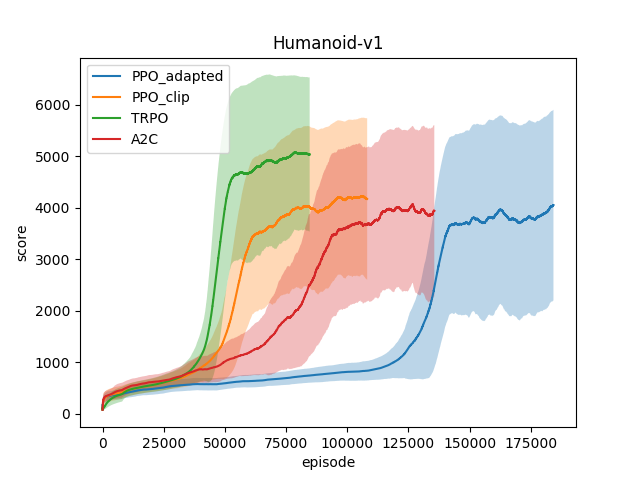
\includegraphics[width=.5\textwidth,height=.5\textheight,keepaspectratio]{Humanoid}
  \end{figure}

  In the above benchmark, we can see that Advantage Actor Critc algorithm is
  able to converge rewards at around 100000 episodes. That tells me that I have to be
  patient on my training and have good metrics to tell if my model will converge
  or not.
  
	\section{Evaluation Metrics}
  \paragraph{}
  I will need two metrics because I have two kind of session for the body: it can walk
  and fail to stand or it can walk without falling. When the avatar will fall, I
  will restart the session, because to teach it to stand up is another kind of
  problem.
  \paragraph{}
  At the beggining of the training, the body will fall and fall again very quickly.
  So my metric during that period will be the amount of restart per second. When the
  body will start to have less fall, that metric will not be informative anymore.
  I have to find metrics to evaluate the gait of the walk. For that, I will plot
  the angle of the current body position from the start position in respect to the
  axe the avatar will try to follow. I will also plot the distance of the gravity
  center from the floor, the mean speed and the reward per action, in order to
  compare with the above benchmark.
  
	\section{Project Design}
  \paragraph{}

  In order to solve that problem, I will first design the architcture of my program
  on paper. The thing is to have a global comprehension of the flow of the program.
  Then I will desgin my model with Keras and Tensorflow, Keras for the simplicity
  and Tensorflow to have my first insight with it. Indeed, I think the simplicity
  of Keras will prevent me to implement properly the model below.

  \begin{figure}[ht]
    \centering
    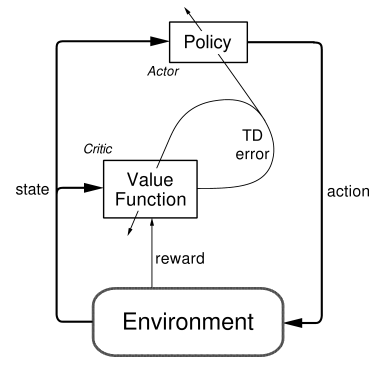
\includegraphics[width=.5\textwidth,height=.5\textheight,keepaspectratio]{actor-critic.png}
  \end{figure}

  For my models, I will use fully-connected layers with not more five 5 hidden
  layers. The powerness of the actor-critc algorithm lies in the team works
  between them and not in their complexity.
  \paragraph{}
  I will design my network for the policy with experience replay, in order to
  feed the actor with a random set of its memory \verb?<state, action, reward, state+1, Q>?
  weighted by the Q-value outputed by the critic network (in order to learn more
  on good actions and less on bad action). The policy will be $\epsilon$-greedy,
  that means it will have an $\epsilon$ chance to take a random action.
  That value will decrease over time to have good exploration-exploitation policy.

  \bibliography{proposal}
  \bibliographystyle{plainnat}
  
  \printglossary
\end{document}
